\definecolor{lavander}{cmyk}{0,0.48,0,0}
\definecolor{violet}{cmyk}{0.79,0.88,0,0}
\definecolor{burntorange}{cmyk}{0,0.52,1,0}

\def\lav{lavander!90}
\def\oran{orange!30}

\tikzstyle{time}=[draw,circle,violet,bottom color=\lav,
                  top color= white, text=violet,minimum width=20pt]
                  
\tikzstyle{base}=[draw,circle,burntorange, left color=\oran,
                       text=violet,minimum width=20pt]

\begin{figure}[h!]
\centering
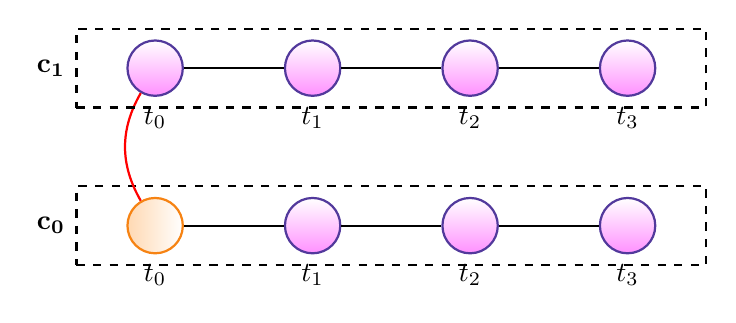
\begin{tikzpicture}[auto, thick]
  \node[base,label=below:$t_0$] (c0t0) at (0,0) {};
  \node[time,label=below:$t_1$] (c0t1) at (2,0) {};
  \node[time,label=below:$t_2$] (c0t2) at (4,0) {};
  \node[time,label=below:$t_3$] (c0t3) at (6,0) {};
  
  \path (c0t0) edge (c0t1);
  \path (c0t1) edge (c0t2);
  \path (c0t2) edge (c0t3);
  
  % rectangle from (-1.0,-0.5) to (7.0,0.5)
   \node[draw,rectangle,dashed,minimum width=8cm,minimum height=1cm,label=left:{$\mathbf{c_0}$}] (s0) at (3.0,0.0) {};
  
  \node[time,label=below:$t_0$] (c1t0) at (0,2) {};
  \node[time,label=below:$t_1$] (c1t1) at (2,2) {};
  \node[time,label=below:$t_2$] (c1t2) at (4,2) {};
  \node[time,label=below:$t_3$] (c1t3) at (6,2) {};
  
  \path (c1t0) edge (c1t1);
  \path (c1t1) edge (c1t2);
  \path (c1t2) edge (c1t3);
  
  \path (c0t0) edge [bend left,color=red] (c1t0);
  
   % rectangle from (-1.0,1.5) to (7.0,2.5)
   \node[draw,rectangle,dashed,minimum width=8cm,minimum height=1cm,label=left:{$\mathbf{c_1}$}] (s0) at (3.0,2.0) {};
  
  
  
%  \foreach \place/\name in {{(0,-1)/a}, {(2,0)/b}, {(2,2)/c}, {(0,2)/d},
%           {(-2,0)/e}}
%    \node[superpeers] (\name) at \place {a};
%  \foreach \source/\dest in {a/b, a/c, a/d, b/c, c/d,a/e,d/e}
%    \path (\source) edge (\dest);
   %
   % Place normal peers
%  \foreach \pos/\i in {above left of/1, left of/2, below left of/3}
%    \node[peers, \pos = e] (e\i) {};
%   \foreach \speer/\peer in {e/e1,e/e2,e/e3}
%    \path (\speer) edge (\peer);
   %
%   \foreach \pos/\i in {above right of/1, right of/2, below right of/3}
%    \node[peers, \pos =b ] (b\i) {};
%   \foreach \speer/\peer in {b/b1,b/b2,b/b3}
%   \path (\speer) edge (\peer);
   %
%   \node[peers, above of=d] (d1){};
%   \path (d) edge (d1);
   %
%   \foreach \pos/\i in {below left of/1, below of/2}
%   \node[peers, \pos =a ] (a\i) {};
%   \foreach \speer/\peer in {a/a1,a/a2}
%   \path (\speer) edge (\peer);

\end{tikzpicture}
\caption{Multi-period contingency constrained optimal power flow example with two contingencies $c_0$ and $c_1$, each with four time-periods $t_0$, $t_1$, $t_2$, $t_3$. State $c_0,t_0$ represent the base case (no contingency) case. We assume that any contingency is incident at the first time-step, i.e., at $t_0$. The contingency states $c_1,t_0$ is coupled with the no-contingency state $c_0,t_0$ at time $t_0$. The {\textcolor{red}{red}} line denotes the coupling between the contingency.}
\label{fig:ctopflow}
\end{figure}